\section{Choosing a Basis to Make Interpolation Easy}

\textbf{(a)}
The values of the signal are linear functions of the sampled values. If
\[
x=
\begin{bmatrix}
y_{t_1}\\ \vdots\\ y_{t_m}
\end{bmatrix}
\]
then linear interpolation constructs a vector \(y=Ax\) for some fixed matrix \(A\). Therefore the set of all signals constructible by linear interpolation is
\[
\mathrm{range}(A)
\]
which is a subspace. Equivalently, linear combinations of interpolated signals are still interpolated signals, since interpolation is linear in the sample values.

\textbf{(b)}
For \(n=20\) and sample times \(1,5,11,20\), the interpolation matrix is
\[
A=
\begin{bmatrix}
1&0&0&0\\
0.75&0.25&0&0\\
0.5&0.5&0&0\\
0.25&0.75&0&0\\
0&1&0&0\\
0&0.8333&0.1667&0\\
0&0.6667&0.3333&0\\
0&0.5&0.5&0\\
0&0.3333&0.6667&0\\
0&0.1667&0.8333&0\\
0&0&1&0\\
0&0&0.8889&0.1111\\
0&0&0.7778&0.2222\\
0&0&0.6667&0.3333\\
0&0&0.5556&0.4444\\
0&0&0.4444&0.5556\\
0&0&0.3333&0.6667\\
0&0&0.2222&0.7778\\
0&0&0.1111&0.8889\\
0&0&0&1
\end{bmatrix}
\]

\begin{figure}[H]
    \centering
    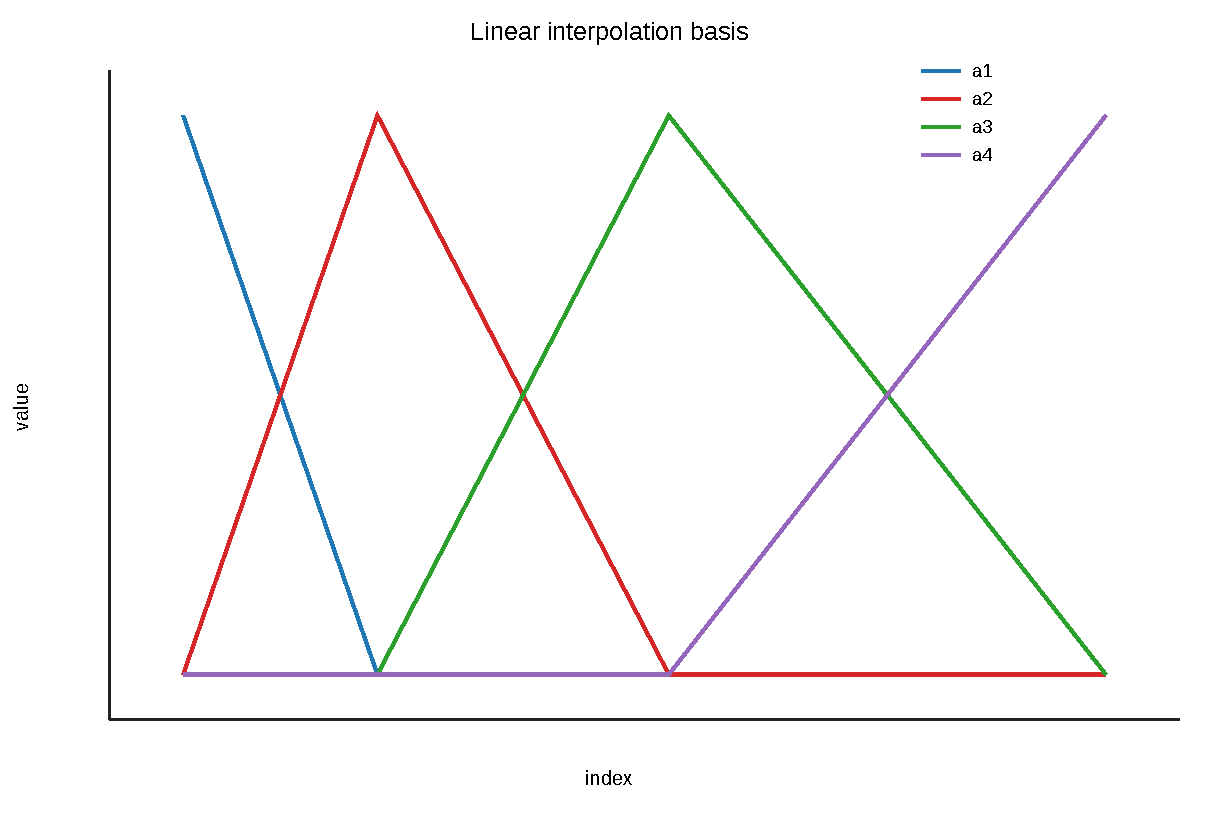
\includegraphics[width=0.82\textwidth]{img/p4_linear_columns.pdf}
    \caption{Columns of the linear interpolation matrix \(A\)}
\end{figure}

\textbf{(c)}
The rank is
\[
\mathrm{rank}(A)=4
\]
The rows of \(A\) at the sample times \(1,5,11,20\) are
\[
e_1^T,\quad e_2^T,\quad e_3^T,\quad e_4^T
\]
so the four columns are linearly independent.

\textbf{(d)}
The simpler algorithm is just to read the sample values out of \(y\):
\[
x=
\begin{bmatrix}
y_1\\y_5\\y_{11}\\y_{20}
\end{bmatrix}
\]
This works because the rows of \(A\) at the sample times form the identity matrix.

\textbf{(e)}
Since the columns of \(B\in\mathbb{R}^{n\times m}\) are a basis for the subspace, \(B\) has rank \(m\). Therefore its rows contain \(m\) linearly independent row vectors. An algorithm for finding the sample times is:

\begin{lstlisting}[language={}]
selected = []
current = empty matrix with m columns
for i = 1:n
    if rank([current; B[i, :]']) increases
        add i to selected
        add B[i, :]' to current
    end
    stop once m rows have been selected
end
\end{lstlisting}

The selected rows form
\[
Z=
\begin{bmatrix}
b_{t_1}^T\\
\vdots\\
b_{t_m}^T
\end{bmatrix}
\]
and by construction \(Z\) is invertible.

\textbf{(f)}
Assume \(v^{(1)},\ldots,v^{(m)}\) is a basis for \(S\), and that
\[
y=v^{(1)}y_{t_1}+\cdots+v^{(m)}y_{t_m}
\]
holds for all \(y\in S\). Set \(y=v^{(i)}\). Then
\[
v^{(i)}
=
\sum_{j=1}^m v^{(j)}v^{(i)}_{t_j}
\]
By uniqueness of coordinates in a basis, the coefficient of \(v^{(j)}\) must be \(1\) when \(j=i\), and \(0\) otherwise. Hence
\[
v^{(i)}_{t_j}
=
\begin{cases}
1,&i=j\\
0,&i\ne j
\end{cases}
\]

\textbf{(g)}
Now assume
\[
v^{(i)}_{t_j}
=
\begin{cases}
1,&i=j\\
0,&i\ne j
\end{cases}
\]
For any \(y\in S\), write
\[
y=\sum_{i=1}^m \gamma_i v^{(i)}
\]
Evaluating at \(t_j\),
\[
y_{t_j}
=
\sum_{i=1}^m \gamma_i v^{(i)}_{t_j}
=\gamma_j
\]
Thus the coordinates of \(y\) in this basis are exactly the sampled values, so
\[
y=\sum_{i=1}^m v^{(i)}y_{t_i}
\]

\textbf{(h)}
Given \(B\) with \(\mathrm{null}(B)=\{0\}\), first select \(m\) independent rows to form the invertible matrix \(Z\). Then define
\[
V=BZ^{-1}
\]
The columns of \(V\) are a basis for \(\mathrm{range}(B)\), since \(Z^{-1}\) is invertible. Also the selected rows satisfy
\[
V_{\{t_1,\ldots,t_m\},:}=ZZ^{-1}=I
\]
so the basis has the desired interpolation property.

\textbf{(i)}
For the given data in \texttt{interp.json}, the algorithm selects
\[
t_1=1,\qquad t_2=2,\qquad t_3=5
\]
The special basis is
\[
V=BZ^{-1}
\]
where \(Z\) is the submatrix formed from rows \(1,2,5\) of \(B\).

\begin{figure}[H]
    \centering
    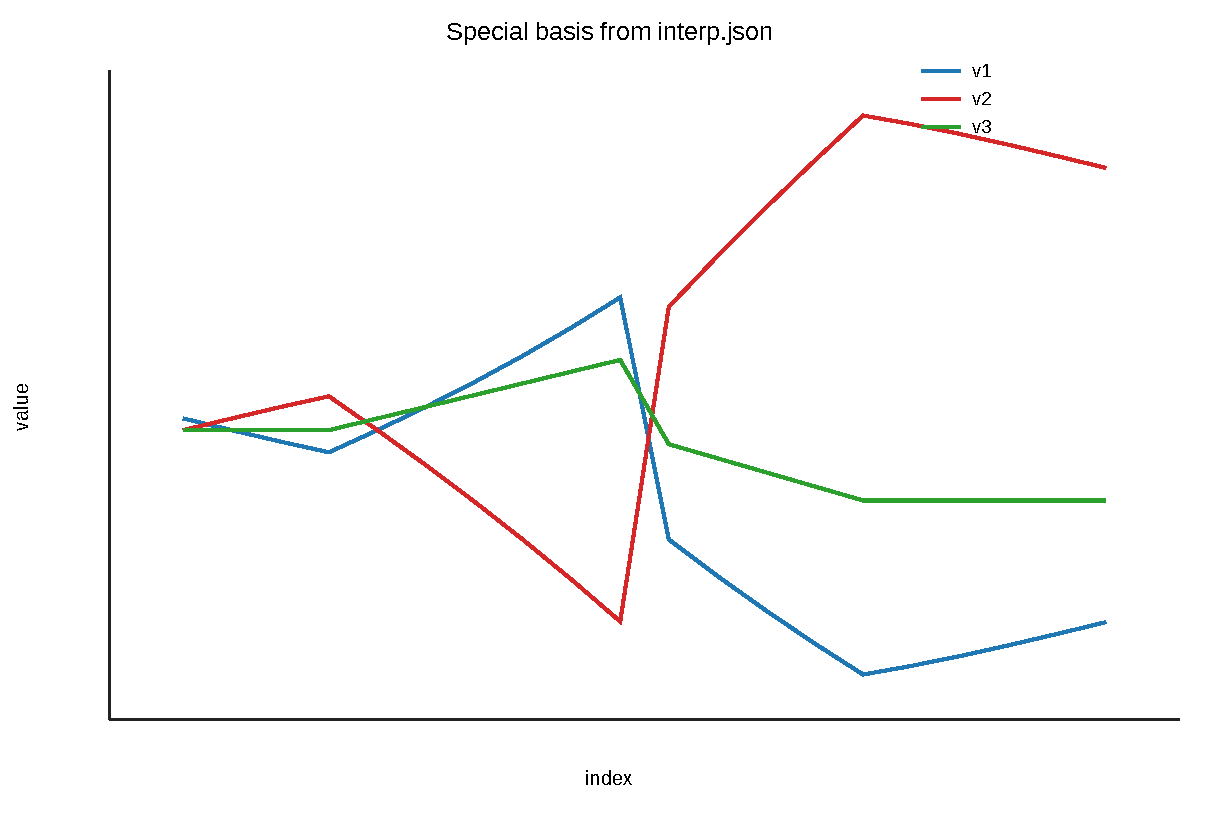
\includegraphics[width=0.82\textwidth]{img/p4_special_basis.pdf}
    \caption{Special basis vectors \(v^{(1)},v^{(2)},v^{(3)}\) for \(\mathrm{range}(B)\)}
\end{figure}

Relevant code:
\lstinputlisting[language={},firstline=6,lastline=43]{../code/p4_interpolation.jl}
\lstinputlisting[language={},firstline=60,lastline=64]{../code/p4_interpolation.jl}
